\section{Methodology} \label{section:background}


In this section, several necessary knowledge is discussed before the reader could understand deeply on our work problem and solution.

\subsection{Spectral Reflectance}
% Challenge:
% It is difficult for the reader to understand about value of input.
% It is potential to bring back enrich information from the spectral reflectance.
% Objective:
% Defition, collective method, enriched information, useful of information.

% What is the spectral reflectance
The reflectance is the effectiveness in reflecting radio energy of a surface,
and different radio wavelength has different reflectance on the same surface.
By combining multiple wavelength reflectance,
we gain a spectral reflectance of the targeted surface.

% Characteristic of reflectance
It is a highlight that different material provides different reflectance spectrum
basing on the material physical characteristics, chemical conditions, or environmental surroundings.
This interesting fact plays a key role in the material recognition through their spectral reflectance.
The hypothesis is that by collecting enough sample reflectance of a surface,
it is possible to analysis a list of materials existed there.
Even more advanced, we could approximately guess about the quantitative of those materials.

Actually, this hypothesis is quite robustness
through a bunch of its application in the astronomy domains.
For instances, the NASA scientists uses the spectral reflectance
to analyze materials existed in a planet, star, or even a galaxy.
Therefore, it is a potential question about its application in the smart agriculture also.

% Move into context
More detail, in this work, we try to examine that question by
an afford to find out the relationship between
the spectral reflectance of the rice leave
with the concentration level of three important chemicals: phosphrus, potassium, and chlorophyll.
Our final target is a quality prediction of these chemicals based on their reflection from the sunlight
which could be easy captured through UAV devices.
However, because of accuracy, in this work context,
we use a high quality device to collect the leave spectral reflectance.
In other words, we manually go to each rice, then capture their leave reflection by an expensive hand device.
This interesting collective method is discussed in other part of report
and be illustrated to our accuracy of their relationship found if having any.




\subsection{Regression Analysis}
% Challenge:
% There is missunderstand point about the usage of Regression method and the useful data extraction on the spectral reflectance.
% Objective:
% Definition, the useful of method on difficult properties of understanding on spectral reflectance.

% What is regression analysis
Regression analysis is a statistical technique for estimating
the relevancy between a dependent variable and one or multiple base variables.
The technique gain this relevancy by applying following steps:
Firstly, researchers a model that is believed to match to the observed samples.
Commonly, the model is a mathematical map/function:

\begin{center}
    $R^{n} \mapsto R$
\end{center}

where $R^{n}$ presents $n$ dimension inputs or base variables
and $R$ presents scalar space of the dependent variable.

In this map, there are also multiple internal parameters of transformation called weights.
The researchers apply their chosen method to estimate these weights values
that satisfies the output of map from the corresponding inputs is approximately resemble of the observed samples.

% Why do we use regression analysis
The model, provided by regression analysis, could be considered as an approximate representation
of the relationship between the dependent variable and its corresponding based variables.
Noting that this statement is only true if the premised model is carefully chosen
and the process weight esitmation go right.
Then, this statistical model is used to examine our understanding on the data,
or applying in the future anticipated of important events.

In our work, this statistical approach is quite potential to analyze our spectral reflectance data.
We have a large amount reflected band/wavelength recored for a rice leave,
and we have a corresponding data of several concerned chemicals data collected directly
from those rice leave through laboratory aproach.
These data relationship are fuzzy
as well as their amount of factors causing difficulty of directly deducing.
Therefore, we try to use several common regression model applying in our data
hoping with luck if the relationship could be discovered here.

\subsubsection{Phosphorus}
Phosphorus (P) is an important nutrient for plants that supports root growth, energy production, storage, and transfer, and produces flowers and fruits. The lack of P can affect negatively the growth and overall health of plants. 

\subsubsection{Potassium}

Potassium (K) is an essential nutrient for plant growth and development. It plays an irreplaceable role in the physiological processes within plants. It helps control tiny openings and closing pores called stomata on the surface of the leaves. It also helps move water and nutrients inside plants. 


\subsubsection{Chlorophyll}

Chlorophyll is a plant’s special reaction that takes part in photosynthesis. It plays an important role in the process of photosynthesis which is how plants convert light energy into chemical energy. Chlorophyll’s green color comes from its ability to absorb light in the blue and red parts of the electromagnetic spectrum while reflecting green\cite*{chlorophyll}.

Chlorophyll-A is a special kind of chlorophyll. It grabs most of the energy from violet-blue and orange-red light but it is not very good at catching green light. Instead of reflecting green light, it mostly uses other colors. Chlorophyll-A is the main pigment that helps plants make food from light. 

\subsubsection{Normalized difference vegetation index (NDVI)}
NDVI is a widely-known measurement for monitoring the health and density of vegetation using sensor data. As introduction, the metric used the spectrometric data at 2 specic bands: red and near-infrared(NIR) for its calculation. Most of thesse spectrometric data is obtained through satellites or in our cases, an UAV Drone. Popularized in the industry, it has been proven to have high correlation with the true state of plants. Determine the 

\begin{quote}
    \(NDVI = \ \frac{NIR - Red}{NIR + Red}\ \)
\end{quote}

Red is a visible light, has a fairly long waves, with wavelegth around 625 to 750nm. Infra-red, however, is an electromagnetic radiation spectrum with wavelegth above red which is between 780 nm and 1mm. Together, they could create thounsands of combination. Data limited by these pairs have many affect on the result of the models. Determine the most compatible pairs for each individual to get the most desirable outcome will be one of the main focus of this study. 


\subsection{Regression Analysis}
% Challenge:
% There is missunderstand point about the usage of Regression method and the useful data extraction on the spectral reflectance.
% Objective:
% Definition, the useful of method on difficult properties of understanding on spectral reflectance.

% What is regression analysis
Regression analysis is a statistical technique for estimating
the relevancy between a dependent variable and one or multiple base variables.
The technique gain this relevancy by applying following steps:
Firstly, researchers a model that is believed to match to the observed samples.
Commonly, the model is a mathematical map/function:

\begin{center}
    $R^{n} \mapsto R$
\end{center}

where $R^{n}$ presents $n$ dimension inputs or base variables
and $R$ presents scalar space of the dependent variable.

In this map, there are also multiple internal parameters of transformation called weights.
The researchers apply their chosen method to estimate these weights values
that satisfies the output of map from the corresponding inputs is approximately resemble of the observed samples.

% Why do we use regression analysis
The model, provided by regression analysis, could be considered as an approximate representation
of the relationship between the dependent variable and its corresponding based variables.
Noting that this statement is only true if the premised model is carefully chosen
and the process weight esitmation go right.
Then, this statistical model is used to examine our understanding on the data,
or applying in the future anticipated of important events.

In our work, this statistical approach is quite potential to analyze our spectral reflectance data.
We have a large amount reflected band/wavelength recored for a rice leave,
and we have a corresponding data of several concerned chemicals data collected directly
from those rice leave through laboratory aproach.
These data relationship are fuzzy
as well as their amount of factors causing difficulty of directly deducing.
Therefore, we try to use several common regression model applying in our data
hoping with luck if the relationship could be discovered here.

\subsection{Dimensionality Reduction}
Dimensionality reduction is a technique aimed at representing a dataset with a reduced number of features (or dimensions) while preserving the essential characteristics of the original data. This process involves the elimination of irrelevant or redundant features, as well as the removal of noisy data, resulting in a model with fewer variables. Dimensionality reduction includes a range of feature selection and data compression methods employed during preprocessing. Although these methods vary in their approaches, they share the common goal of transforming high-dimensional spaces into low-dimensional ones through the extraction or combination of variables.

\subsection{Scikit-learn}
Scikit-learn is an open-source machine learning library for python
which supports vast amount of data analysis and machine learning algorithms.
It propose many utilities components and tools to interact with machine leanring tasks
like classification, clustering, and regression analysis
as well as data preprocessing tasks like dimension reduction, null data cleaner, etc.

Besides, it is notable that Scikit-learn is designed to interoperate
with others populer strongly python library and framework
as Numpy (algebraic computation framework) or Scipy (signal computation framework).
It allows to transperantly develope a full data processing pipeline
with minimal effort on convesion.

In our work, the experiment on different aspect of data is necessary
to discover any potential relation between reflectance data to the concetrate level of NPK chemicals.
So, for productivity, a universal and reliable framework like Scikit-learn
which proposes multiple predefined data analytics solutions readily to apply into an expected data
is an irreplaceable option.

%\son{move to method}

\subsection{PCA}
PCA is a method used to reduce the dimensionality of the dataset by transforming variables into smaller ones but still contains important features of the dataset. 
Principal components are variables represented as linear combinations of the initial elements in the dataset.
the dataset after simplification is easier to understand and easier to visualize. Various fields of science have already applied PCA to their data like genetics or climate science where it reduces the complexity of the data\cite*{pca}.

This is how the PCA works step-by-step:

\paragraph*{Step 1: Standardization}
In this step, the goal is to standardize the variables to have the same impact on the analysis by their ranges. This is a necessary step when PCA. If some variables have much larger ranges, they can unfairly dominate the results. Standardizing involves adjusting data to a common scale by subtracting the average and dividing by the standard deviation for each value of each variable. 
\begin{quote}

\(z = \frac{value - mean}{standard\ deviation}\)
\end{quote}

\paragraph*{Step 2: Covariance matrix computation}
This step is to find connections between variables by comparing how they change from their average to each other. This helps spot repeated info. We use the covariance matrix for this

\begin{quote}

\(cov(X,Y) = \ \frac{1}{n}\ \sum_{i=1}^{n}\left( X - \ \underline{X} \right)\left( Y - \ \underline{Y} \right)\)
\end{quote}

\begin{itemize}
    \item cov(X, Y) is the covariance between X \& Y variables
    \item x \& y are members of X and Y variables
    \item \(\underline{x}\) and\(\ \underline{y}\) are mean of X \& Y variables
    \item n is the number of members 
\end{itemize}

It’s a chart that shows how variables connect based on their changes. For example, in 3D data with x, y, and z variables, the covariance matrix is a 3x3 grid. 
\begin{quote}
    \begin{bmatrix}
        \text{Cov}(x,x) & \text{Cov}(x,y) & \text{Cov}(x,z) \\
        \text{Cov}(y,x) & \text{Cov}(y,y) & \text{Cov}(y,z) \\
        \text{Cov}(z,x) & \text{Cov}(z,y) & \text{Cov}(z,z)
    \end{bmatrix}
\end{quote}
    
The diagonal of the matrix shows each variable’s variance because a variable’s covariance with itself is its variance (Cov(a, a)=Var(a)). Moreover, due to the commutative property of covariance (Cov(a,b)=Cov(b, a)), the covariance matrix is symmetric which means that the upper and lower triangular sections mirror each other across the main diagonal.

\paragraph*{Step 3: Eigenvectors and eigenvalues}
Eigenvectors and eigenvalues are linear algebra concepts used to compute from the covariance matrix to determine the principal components of the data. Because these two values always connect in pairs and their number is equal to the dimensions of the data. 

The eigenvectors of the covariance matrix contain the most variance of the data and that is called principal components. The eigenvalues are the coefficients of the eigenvectors and thus represent the amount of variance in each principal component.

This step process primarily removes ignorable components while keeping the significant variables and convert into new variables. The principle components indicate the directions of the data.
\begin{quote}
    
    \(Av = \ \lambda v\)
\end{quote}
\begin{itemize}
    \item A is the matrix
    \item V is a special vector
    \item \(\lambda \) is an eigenvalue
\end{itemize}

This step process primarily removes ignorable components while keeping the significant variables and convert into new variables. The principle components indicate the directions of the data.
The importance of the principal components can be determined by ordering the eigenvectors by their eigenvalues decreasing.

\paragraph*{Step 4: Feature vector}
By computing and sorting eigenvectors by their eigenvalues, we identify principal components in order of importance. The feature vector is a matrix formed from the chosen eigenvectors, serving as the first step in dimensionality reduction. Selecting p eigenvectors out of n reduces the dataset to p dimensions. 

\paragraph*{Step 5: Reorient the principal components axes}

\begin{quote}
    \(FinalDataSet = {FeatureVector}^{T}*\ {StandardizedOriginalDataSet}^{T}\)
\end{quote}
Throughout the first 4 steps, The data only had been standardiazation without any others change and only select the principal components of the data and the data still remains in the same original axes.
Lastly, we aim to reorient the data from the original axes into a new axes which represented by the principal components.

Our dataset in this project is pretty large and contains a high number of dimensions, so we apply PCA to reduce the dimension and increase the model’s efficiency. To find the best number of components that will be well-suited to the data, we use the result of the explained variance and the cumulative variance The figure below shows the information on the explained variance of the dataset. 


\begin{figure}[h]
    \centering
        \subfigure[]{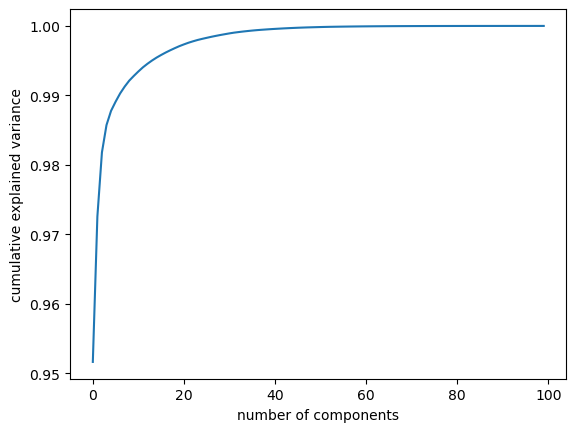
\includegraphics[width=0.7\textwidth]{image/pca.png}}
    \caption{The number of components needed to explain variance
    } \label{fig:no-component-variance}
\end{figure}
From the figure, five number of component should be enough to get most of the dataset variance coverage, 
\subsection{Machine Learning}

\subsubsection{Ridge}
Ridge regression is also a technique used in linear regression, the same as lasso, which is a tool that helps fix tuning models when dealing with closely related data, called a multicollinearity problem\cite{ridge}. It applies L2 regularization to handle this. When data has multicollinearity, standard least-square techniques stay unbiased, but variation grows, which leads to substantial differences between predicted parameter estimation. To deal with this, ridge regression adds some bias to improve the accuracy with which parameters are estimated.
The cost function for ridge regression can be performed like this: 
\begin{quote}
    
    \(J(\theta) = \frac{1}{2m}\sum_{i=1}^{m}((h_{\theta}(x^{(i)} - {y^{(i)})}^{2} + \lambda\sum_{j=1}^{n}\left| \theta_{j} \right|)\)
\end{quote}
    
\begin{itemize}
    \item \(J(\theta)\): cost function
    \item \(m\) number of the training set
    \item \(h_{\theta}(x^{(i)}\)\textbf{)}: predicted output value of
    i\textsuperscript{th} training examples
    \item \(\lambda\): regularization term,
    \item \(n\): number of features,
    \item \(\theta_{j}\): weight of j\textsuperscript{th} feature.

\end{itemize}

Ridge regression works best when having more predicted variables than the observations in the data. This is especially useful in cases where the standard assumptions of linear regression might not be valid. It finds a middle ground between effectively capturing relationships within the data and preventing overfitting issues. 

\subsubsection{Lasso}

Lasso regression is a technique used in regression analysis. Like Ridge Regression, it is a way to shrink and select coefficients in linear regression models, especially with many predictors or multicollinearity. It adds a penalty based on absolute coefficient values ( L1 regularization), which can precisely zero out some coefficients. Effectively performing feature selection. This prevents overfitting, simplifies models, and is great when only a subset of predictors is vital.
\begin{quote}
    
    \(J(\theta) = \frac{1}{2m}\sum_{i=1}^{m}((h_{\theta}(x^{(i)} - {y^{(i)})}^{2} + \lambda_{1}\sum_{j=1}^{n}\theta_{j}^{2} + \lambda_{2}\sum_{j=1}^{n}\theta_{j}^{2})\)
\end{quote}

\begin{itemize}
    \item \(J(\theta)\): cost function
    \item \(m\): number of the training set
    \item \(h_{\theta}(x^{(i)}\)\textbf{)}: predicted output value of
    i\textsuperscript{th} training examples
    \item \(\lambda\): regularization term,
    \item \(n\): number of features,
    \item \(\theta_{j}\): weight of j\textsuperscript{th} feature.

\end{itemize}

What makes Lasso different from Ridge is that while Lasso can lead to zero coefficients, Ridge keeps predictors, although their magnitude is reduced. By ignoring some specific predictors, Lasso is best for its simplicity and clarity, whereas Ridge is well-suited for situations where numerous influential predictors are involved

\subsubsection{ElasticNet}

ElasticNet is a powerful and flexible regularization method which have both characteristics of Lasso and Ridge regression, it merges the capability of dealing with high-dimensionality and the need for robust regularization techniques which means that ElasticNet is the combination of L1 and L2 regularization. By mixing L1 and L2 regularization, it aims to strike a balance between simplicity and retaining relevant predictors. ElasticNet provides two parameters, alpha, and lambda, to balance these two types of regularization. The alpha parameter controls the mix of L1 and L2 regularization, allowing us to emphasize one over the other or find an equilibrium between the two. The lambda parameter controls the overall strength of regularization, controlling how much the coefficients shrink

\begin{quote}
    
    \(J(\theta) = \frac{1}{2m}((h_{\theta}(x^{(i)} - {y^{(i)})}^{2} + \lambda_{1}\theta_{j}^{2} + \lambda_{2}\theta_{j}^{2})\)
\end{quote}


\begin{itemize}
    \item \(J(\theta)\): cost function
    \item \(m\): number of the training set
    \item \(h_{\theta}(x^{(i)}\)\textbf{)}: predicted output value of
    i\textsuperscript{th} training examples
    \item \(y^{(i)}\): real output value of ith training examples,
    \item \(\lambda_{1}\)\textbf{,} \({\ \lambda}_{2}\):: regularization terms,
    \item \(n\): number of features,
    \item \(\theta_{j}\): weight of jth feature.
\end{itemize}

\subsubsection{Decision Tree}
Decision tree is a versatile algorithm used for classification and regression tasks\cite{DecisionTree}. A decision tree is a supervised learning technique mainly applied for classification task machine learning, where the data is represented in a tree-like structure. 

The Decision tree components include Root Node which is the whole dataset where the tree starts. From the root node, the tree will be divided into a subtree known as decision nodes. At the end of a branch will be a leaf node and cannot be split into another branch.

The main advantage of using the decision tree is the algorithm works like a human thinks and makes decisions and is easy to understand due to the tree-like structure. this approach also requires fewer resources to pre-process than other algorithms. However, the number of branches is higher the more complex the data is and contains lots of layers. The bigger the tree, the more the output will be overfitting.

Pruning - With a big tree model, to prevent the data from overfitting, the data will be pruned which is a process to remove branches containing non-important decisions/output of the tree. Cost complexity pruning and reduced error pruning are the most well-known processes. The other known way to reduce the chance of overfitting is using a random forest algorithm.


\begin{figure}[h]
\centering
    \subfigure[]{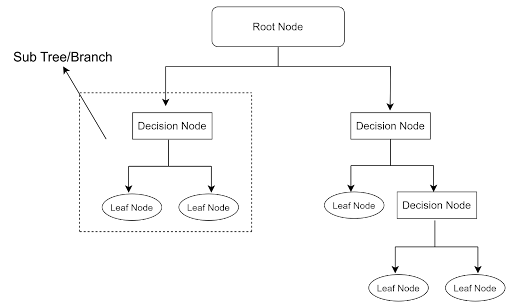
\includegraphics[width=1\textwidth]{image/decision_tree_workflow.png}}
\caption{Decision Tree workflow} \label{fig:decision-tree-workflow}
\end{figure}


The decision tree starts with data preparation, where a dataset with input features and a target variable is collected. It selects initial features as the root node, splits the data based on feature values, and calculates the reduction at each step. When the process chooses the best split, which will become the first split of the tree, it will repeat from the beginning to this step. To make predictions, it goes from branches based on feature values to reach leaf nodes, which contain target value predictions that have averaged. After evaluation with metrics like MSE or R squared, it may apply pruning to refine the tree’s structure. 

\subsubsection{Random Forest}
Random forest is a learning method for regression or classification tasks that construct a decision tree when training \cite{randForest}. 
The random forest algorithms train data while applying the technique of bootstrap aggregating to tree branches to deal with an uncorrelated ensemble of the decision trees. this technique will make sure that each decision tree in the forest is set for a different set of features, by randomly selecting a subset of features from the dataset. 


\begin{figure}[h]
\centering
    \subfigure[]{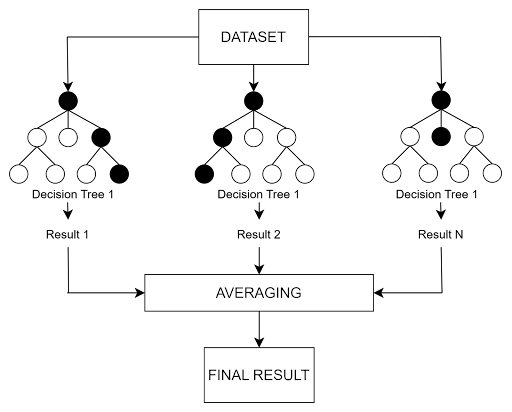
\includegraphics[width=1\textwidth]{image/rand_forrest_workflow.png}}
\caption{Random Forest workflow} \label{fig:rand_forrest_workflow}
\end{figure}

The Random Forest algorithm runs through a bunch of systematic steps to create a predictive model. It starts with data preparation and then uses bootstrapping to create diverse subsets of the data. For each subset, it constructs a decision tree that contains information about the feature randomness, which means that there is only a random subset of features at each node for splitting. Predictions from these trees are combined through averaging for regression and voting for classification to get to the final prediction. The Random Forest model can be working great through parameter adjustments and evaluated using suitable metrics, while also giving a view of feature importance. 

Random Forest brings users several advantages such as their versatility and accuracy when handling diverse data types including binary, numerical, and categorical features, making them robust against outliers and nonlinear features. One of the most useful capabilities is its ability to balance errors in populations and unbalanced datasets, measuring feature importance is straightforward. However, they can be slower due to building many trees, limiting real-time use. The predictions rely on past data and may not work well with different ranges. Also, they are not easy to understand and the decisions cannot be explained easily.

\subsubsection{Support Vector Regression}
Support Vector Regression (SVR) is a specialized type of support vector machine (SVM) used for regression tasks, targeted to predict continuous output values based on given input data. It can be used both for linear and non-linear kernels, with a simple dot product between input vectors for linear kernels while capturing more complex data patterns for non-linear kernels. Choosing between linear and non-linear is based on data characteristics and task complexity. SVR is based on SVM principles, with the same main role being error minimization while finding a hyperplane with a margin that allows for some error. 
This minimization process for the parameter ‘w’ in the equation is akin to maximizing the margin:
\begin{quote}
    \({\min\left| |w| \right|}^{2} + C\sum_{i}^{n}(\xi_{i}^{+} + \ \xi_{i}^{-})\ \ \)
\end{quote}

In order to reduce this error, we utilize the following equation, where the summation component represents an empirical error. 


To minimize the error, we use the following equation:
\begin{quote}
    \(f(x) = \ \sum_{i}^{n}\left( \alpha_{i}^{*} + \ \alpha_{i} \right)K\ \left( x,x_{i} \right) + B\)
\end{quote}
And to calculate the kernel K we can use the following equation: 

\begin{quote}
    \(K\left( x,x_{i} \right) = \ \gamma\left( x*\ x_{i} + 1 \right)^{d}\ \)

\end{quote}

Research with other algorithms shows that SVR acquires better results when working with Linear Regression or ElasticNet. The algorithms also show high accuracy results when working with large datasets with a high number of variables. The SVR has high compatibility when used alongside functions such as geometric, transmission, or data generalization.  Implement standardization is highly recommended when ensuring unbiases evaluations.

\subsubsection{Bayesian Ridge}
Bayesian linear regression predicts the mean of one variable using a weighted sum of others. Its goal is to calculate the posterior probability of regression coefficients and other distribution parameters based on observed predictors.  Bayesian regression suits datasets with sparse or poorly distributed data, as it derives the posterior distribution of model parameters rather than estimating them directly. 
\begin{quote}
    \(p(y\ |\ X,w,a)\  = \ N\ (y\ |\ X_{w}{,a)}_{}\)
\end{quote}
Bayesian Ridge regression, which is the most widely used type of Bayesian regression, models regression problems by incorporating probability estimates. This helps account for uncertainty in predictions, making it useful for situations with limited data or noise. The prior for the coefficients w is given by spherical Gaussian as follows.

\begin{quote}
    \(p(w\ |\ \lambda)\  = \ N\ (w\ |\ 0,\ \lambda^{- 1}I_{p}\))
\end{quote}

\subsubsection{Lasso Lars}
Lasso Lars regression is the mixture of two techniques: Lasso and Lars. 
\paragraph{Lasso} is primarily used for feature selection and addressing multicollinearity in linear regression models. On the other hand, Lars is an algorithm used for efficiently selecting variables in a high-dimensional dataset. Combining these two techniques, Lasso Lars inherits the feature selection capabilities of Lasso and the efficient variable selection process of Lars. This makes it particularly well suited for linear regression tasks involving datasets with many predictor variables or situations where multicollinearity is present. 
It starts with all coefficients at zero and selects predictors based on their correlation with the target variable. As it progresses, it employs Lasso’s feature selection, encouraging some coefficients to become zero, simplifying the model. This approach excels in handling high-dimensional data efficiently while building interpretable and accurate linear regression models.

\paragraph{Lars}

Least Angle Regression (Lars) is used for feature selection and model building, which is specially designed for high dimensional datasets. Its main task is to select and incorporate the most correlated contributions into the model without overfitting. To fit the models, we start by normalizing all values. Then we choose the most highly correlated variable with the residual and adjust the regression line. This process continues until we have used all data or created a satisfactory model. 


\begin{figure}[h]
\centering
    \subfigure[]{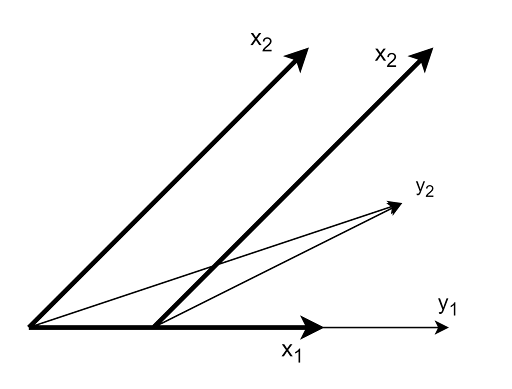
\includegraphics[width=0.8\textwidth]{image/lars.png}}
\caption{Lars Skrinkage} \label{fig:lars}
\end{figure}

\begin{itemize}
    \item y2 is the projection of  y onto L( x1, x2) 
    \item Two covariates x1 and x2 and the space L(x1, x2) that is spanned by them 
    \item Start at \(\mu_{0} = 0\)
\end{itemize}

Firstly, we start with all coefficients as zero and find the predictor variable xj that correlates most with the target variable y. Then we increase the coefficients Bj in the direction of this correlation until another predictor variable xk with equal or higher correlation is found. The coefficients (Bj, Bk) are adjusted so that they have the same angle with xj and xk. This process continues until all predictor variables are included in the model. 

\subsubsection{Boosting}
Boosting is a powerful ensemble meta-algorithm in machine learning that reduces bias and variance in supervised learning. It transforms weak learners into strong ones by combining them iteratively and adjusting their weights based on accuracy. Boosting emerged from the idea of enhancing weak learners to create strong ones. Boosting methods assume training weak classifiers sequentially, making it an essential concept in machine learning and statistics. By each stage of adding, a process called ‘re-weighting’, misclassified data points to gain higher weight, allowing weak learners to focus on them. There are a large number of types of boosting algorithms but in this project, we are supposed to use just the most popular which are AdaBoost, XGBoost, LGBM, CatBoost, and GradientBoost. 


\begin{figure}[h]
\centering
    \subfigure[]{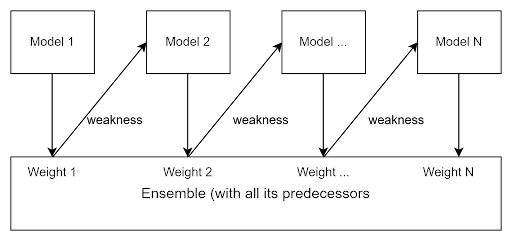
\includegraphics[width=1\textwidth]{image/Boost_workflow.png}}
\caption{Boosting algorithm workflow} \label{fig:Boost_workflow}
\end{figure}


The boosting algorithm contains several advantages, including improved accuracy achieved by combining predictions from weak models, robustness against overfitting by giving more weight to misclassified data points, and effective handling of imbalanced datasets. However, boosting algorithms also have some limitations which can be named as the sensitivity which will make them less suitable when working with real-time applications. Unlike others focused on high-quality predictions, boosting algorithms rely on weak models, each addressing the predecessor’s weaknesses. 


\subsubsection{Gradient Boosting}
Gradient Boosting is a robust boosting algorithm that combines weak learners into strong ones by training each new model to minimize the loss function of the previous model using gradient descent. In each iteration, it calculates the gradient of the loss function regarding the predictions of the current ensemble and trains a new weak model to minimize this gradient. This method often uses decision trees as weak learners to transform the data. The iterative procedure involves computing residuals, which represent the difference between predictions and actual values, and training models to map features to these residuals. These steps are to improve the overall predictive performance of the model. 

We can express how GradientBoosting works through these steps: 

\paragraph*{Step 1:} Assume X and Y are the input and target with N samples. The goal is to find a function f(x) that maps input features X to target variables Y. The loss function quantifies the difference between actual and predicted values
\begin{quote}
    
    \(L(f) = \ \sum_{i=1}^{N}L(y_{i},\ f\left( x_{i} \right))\)
\end{quote}

\paragraph*{Step 2:} Focuses on minimizing L(f) with respect to f
f0x=argmin f  Lf= argmin f  i=1NL(yi, fxi)
In our gradient boosting algorithm with M stages, we improve the model fm by introducing additional estimators denoted as hm, where m ranges from 1 to M
\begin{quote}
    \({\widehat{f}}_{0}(x) = argmin\ f\ \ L(f) = \ argmin\ f\ \ \sum_{i=1}^{N}L(y_{i},\ f\left( x_{i} \right))\)

\end{quote}

\paragraph*{Step 3:} Steepest Descent
\begin{quote}
    \(g_{im} = \  - {\lfloor\frac{\partial L(y_{i},\ f\left( x_{i} \right))}{\partial f(x_{i})}\rfloor}_{f\left( x_{i} \right) = \ f_{m - 1}\ (x_{i})}\)

\end{quote}

With the M stage of Gradient Boosting, the Steepest Descent technique is used to determine the  hm which is an important component. This is the combination of 2 elements: constant termed as step length, and the gradient of the loss function gm. The key point of the step length is to scale the gradient of the loss function L(f). 

\paragraph*{Step 4:} we update the solution iteratively using 
\begin{quote}
    \(f_{m}(x) = \ f_{m - 1}(x) + \left( argmin\ h_{m \in H}\ \ \left\lbrack \sum_{i=1}^{N}L\left( y_{i},\ f_{m - 1}\left( x_{i} \right) + \ h_{m}\left( x_{i} \right) \right) \right\rbrack \right)(x)\)
    
\end{quote}
This process continues for M trees, refining the model at each stage to achieve a more accurate prediction. The solution can also be written as:
\begin{quote}
    \(f_{} = \ f_{m - 1} - \ \rho_{m}g_{m}\)

\end{quote}


\subsubsection{Adaptive Boosting}
AdaBoost, short for Adaptive Boosting is a machine learning algorithm that combines the outputs of weak learners to create a strong classifier. It is known for its adaptability and the ability to handle various base learners including weak ones like decision stumps or even strong learners like deep decision trees, making it versatile. AdaBoost adapts by giving more emphasis to instances that previous learners misclassified, reducing the risk of overfitting. It assigns different weights to errors, influencing the importance of weak learners in the final model. 
This is an example of how AdaBoost works through a pseudocode: 

\begin{quote}
\begin{longtable}[]{@{}
  >{\raggedright\arraybackslash}p{(\columnwidth - 2\tabcolsep) * \real{0.1232}}
  >{\raggedright\arraybackslash}p{(\columnwidth - 2\tabcolsep) * \real{0.8768}}@{}}
\toprule()
\begin{minipage}[b]{\linewidth}\raggedright
\textbf{Input:}
\end{minipage} & \begin{minipage}[b]{\linewidth}\raggedright
Data set
\(D = \left\{ \left( x_{1},\ y_{1} \right),\ \left( x_{2},\ y_{2} \right),\ \ldots\ \left( x_{m},\ y_{m} \right) \right\};\)
\end{minipage} \\
\begin{minipage}[b]{\linewidth}\raggedright
\end{minipage} & \begin{minipage}[b]{\linewidth}\raggedright
Base learning algorithm \(L\);
\end{minipage} \\
\multicolumn{2}{@{}>{\raggedright\arraybackslash}p{(\columnwidth - 2\tabcolsep) * \real{1.0000} + 2\tabcolsep}@{}}{%
\begin{minipage}[b]{\linewidth}\raggedright
\textbf{Output:} \(H(x) = sign(\sum_{t=1}^{T}\alpha_{t}h_{t}(x)\)
\end{minipage}} \\
\begin{minipage}[b]{\linewidth}\raggedright
\end{minipage} & \begin{minipage}[b]{\linewidth}\raggedright
Number of learning round T.
\end{minipage} \\
\begin{minipage}[b]{\linewidth}\raggedright
\textbf{Process:}
\end{minipage} & \begin{minipage}[b]{\linewidth}\raggedright
\end{minipage} \\
\multicolumn{2}{@{}>{\raggedright\arraybackslash}p{(\columnwidth - 2\tabcolsep) * \real{1.0000} + 2\tabcolsep}@{}}{%
\begin{minipage}[b]{\linewidth}\raggedright
\(D_{1}(i) = 1/m\) \% Initialize the weight distribution
\end{minipage}} \\
\multicolumn{2}{@{}>{\raggedright\arraybackslash}p{(\columnwidth - 2\tabcolsep) * \real{1.0000} + 2\tabcolsep}@{}}{%
\begin{minipage}[b]{\linewidth}\raggedright
for \(t = 1,\ \ldots\ ,\ T\);
\end{minipage}} \\
\begin{minipage}[b]{\linewidth}\raggedright
\end{minipage} & \begin{minipage}[b]{\linewidth}\raggedright
\(h_{t} = \ L\left( D,\ D_{t} \right);\ \ \) \% Train a weak learner
\(h_{t}\) from D using distribution \(D_{t}\)
\end{minipage} \\
\begin{minipage}[b]{\linewidth}\raggedright
\end{minipage} & \begin{minipage}[b]{\linewidth}\raggedright
\(\epsilon_{t} = \ \Pr_{i\sim Di}\lbrack h_{t}(x_{i}\  \neq \ y_{i})\rbrack;\)
\% Measure the error of \(h_{t}\)
\end{minipage} \\
\begin{minipage}[b]{\linewidth}\raggedright
\end{minipage} & \begin{minipage}[b]{\linewidth}\raggedright
\(\alpha_{t} = \ \frac{1}{2}\ln\ln\ \left( \frac{1 - \ \epsilon_{t}}{\epsilon_{t}} \right)\ ;\)
\% Determine the weight of the \(h_{t}\)
\end{minipage} \\
\begin{minipage}[b]{\linewidth}\raggedright
\end{minipage} & \begin{minipage}[b]{\linewidth}\raggedright
\(D_{t + 1} = \ \frac{D_{t}(i)}{Z_{t}}\  \times \{\exp\ \left( - \alpha_{t} \right)\ \ if\ h_{t}\left( \ x_{i} \right) = \ y_{i}\ exp\ \left( \alpha_{t} \right)\ \ if\ h_{t}\left( \ x_{i} \right)\  \neq \ y_{i}\ \ \ \ \)

\(= \ \frac{D_{t}(i)exp( - \alpha_{t}y_{i}h_{t}(x_{i})}{Z_{t}}\) \%
update the distribution, where \(Z_{t}\) is

\% a normalization factor which enables \(D_{t + 1}\) be a distribution end.

\end{minipage} \\
\multicolumn{2}{@{}>{\raggedright\arraybackslash}p{(\columnwidth - 2\tabcolsep) * \real{1.0000} + 2\tabcolsep}@{}}{%
\begin{minipage}[b]{\linewidth}\raggedright
\end{minipage}} \\
\midrule()
\endhead
\bottomrule()
\end{longtable}
\end{quote}

AdaBoost offers several advantages, notably its ease of use with minimal parameter tuning, in contrast to more complex algorithms like SVM. However there are some disadvantages, AdaBoost’s progressive learning process demands high-quality data as it’s sensitive to noise and outliers. 


